%\chapter{Hướng dẫn sử dụng template}
\chapter{Phương pháp}
\label{Chapter3}

\section{Mạng lượng tử hoá tích trực chuẩn cho truy xuất ảnh khuôn mặt quy mô lớn}
\subsection{Tổng quan về mạng lượng tử hoá tích trực chuẩn}
Mạng lượng tử hoá tích trực chuẩn là một mạng nơ-ron sử dụng lượng tử hoá với ràng buộc vuông góc, sử dụng bộ mã được định nghĩa trước nhằm tăng độ phân biệt và giảm sự dư thừa giữa các thông tin đặc trưng với nhau, giải quyết các thách thức về biến đổi nội lớp như tư thế, ánh sáng, biểu cảm. Khả năng tổng quá hoá cao, phù hợp với nhu cầu truy xuất các danh tính chưa từng thấy.

\begin{figure}[htbp] % hoặc [htbp]
    \centering
    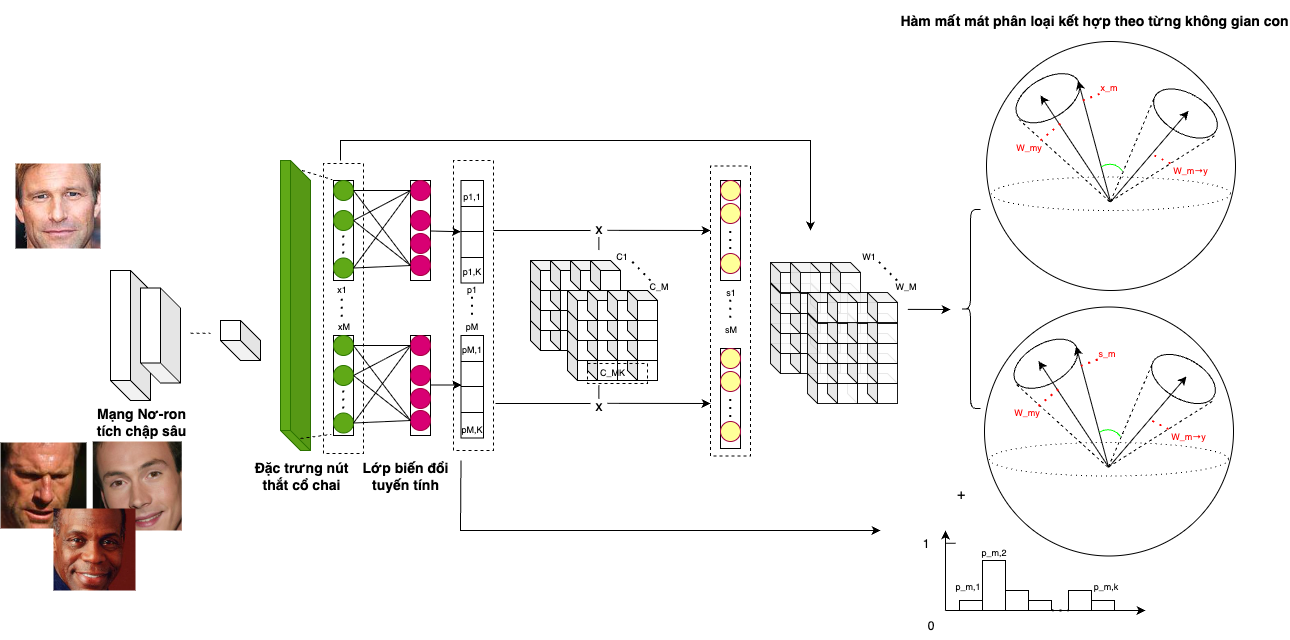
\includegraphics[width=0.8\textwidth]{images/opqn_model.png} 
    \caption{Mô hình lượng tử hoá tích trực chuẩn}
    \label{fig:opqn_rmodel_types}
\end{figure}

Các thành phần chính và kiến trúc của mạng lượng tử hoá tích trực chuẩn bao gồm các thành phần cốt lõi như sau: Mạng xương sống, lượng tử hoá mềm thông qua khử tương quan đặc trưng - xác suất, sinh mã từ trực chuẩn, hàm mất mát phân loại kết hợp theo từng không gian con, tối thiểu hoá độ cô đặc cho việc gán mã one-hot, quá trình học và tối ưu hoá và khoảng cách bất đối xứng trong truy xuất.
\subsection{Các ký hiệu và ký pháp}
Trong mô hình OPQN, các ký hiệu và ký pháp được định nghĩa để mô tả rõ ràng các thành phần dữ liệu, đặc trưng, và hàm mất mát. Bảng \ref{tab:terms_part1} và \ref{tab:terms_part2} trình bày chi tiết các ký hiệu này, được sử dụng xuyên suốt phần phương pháp để giải thích quy trình lượng tử hóa và tối ưu hóa.

\begin{table}[h!]
    \centering
    \begin{tabular}{|c|p{3cm}|p{6cm}|}
        \hline
        \textbf{Ký hiệu} & \textbf{Ký pháp} & \textbf{Mô tả} \\ \hline
        $I_i$ & $\{I_i\}_{i=1}^N$ & Tập hợp $N$ hình ảnh khuôn mặt đầu vào. \\ \hline
        $y_i$ & $y \in \mathbb{R}^N$ & Nhãn danh tính tương ứng với hình ảnh $I_i$. \\ \hline
        $x_i$ & $x_i = f(\Theta, I_i) \in \mathbb{R}^D$ & Đặc trưng nút cổ chai được trích xuất từ hình ảnh $I_i$ bởi mạng xương sống với tham số $\Theta$, có chiều $D$. \\ \hline
        $x_{im}$ & $x_{im} \in \mathbb{R}^d$ & Vector con thứ $m$ của ảnh đặc trưng $x_i$, với $d = D/M$ và $m = 1, \dots, M$. \\ \hline
        $M$ & $M$ & Số lượng vectơ con mà đặc trưng $x_i$ được chia thành. \\ \hline
        $d$ & $d = D/M$ & Chiều của mỗi vector con $x_{im}$. \\ \hline
        $C$ & $C = [C_1, \dots, C_M]$ & Tập hợp $M$ bộ mã, mỗi bộ mã $C_m \in \mathbb{R}^{d \times K}$ chứa $K$ từ mã trực chuẩn. \\ \hline
        $C_{mk}$ & $C_{mk} \in \mathbb{R}^d$ & Từ mã thứ $k$ trong bộ mã $C_m$. \\ \hline
        $F$ & $F = [F_1, \dots, F_M]$ & Tập hợp ma trận tham số của các lớp tuyến tính, với $F_m \in \mathbb{R}^{d \times K}$. \\ \hline
        $F_{mk}$ & $F_{mk} \in \mathbb{R}^d$ & Vectơ tham số thứ $k$ trong ma trận $F_m$. \\ \hline
        $p_{im}$ & $p_{im} = [p_{im,1}, \dots, p_{im,K}] \in \mathbb{R}^K$ & Vector xác suất của vector con $x_{im}$, được tính qua softmax: $p_{im,k} = \frac{e^{x_{im}^T F_{mk}}}{\sum_{j=1}^K e^{x_{im}^T F_{mj}}}$. \\ \hline
        $s_{im}$ & $s_{im} = \sum_{k=1}^K p_{im,k} \cdot C_{mk}$ & Lượng tử hóa mềm của vectơ con $x_{im}$. \\ \hline
        $h_{im}$ & $h_{im} = C_{m k^*}$, $k^* = \arg\max_k p_{im,k}$ & Lượng tử hóa cứng của vectơ con $x_{im}$. \\ \hline
    \end{tabular}
    \caption{Phần 1: Ký hiệu và ký pháp (Dữ liệu và đặc trưng)}
    \label{tab:terms_part1}
\end{table}

\begin{table}[h!]
    \centering
    \begin{tabular}{|c|p{6cm}|p{5cm}|}
        \hline
        \textbf{Ký hiệu} & \textbf{Ký pháp} & \textbf{Mô tả} \\ \hline
        $W$ & $W = [W_1, \dots, W_M]$ & Tập hợp trọng số của các bộ phân lớp theo không gian con, với $W_m \in \mathbb{R}^{d \times C}$. \\ \hline
        $W_{mc}$ & $W_{mc} \in \mathbb{R}^d$ & Trọng số của lớp $c$ trong bộ phân lớp $W_m$. \\ \hline
        $L_x$ & $L_x = \sum_{i=1}^N \sum_{m=1}^M -\log \frac{e^{r (\cos \theta_{y_i, x_{im}} - u)}}{e^{r (\cos \theta_{y_i, x_{im}} - u)} + \sum_{j \neq y_i} e^{r \cos \theta_{j, x_{im}}}}$ & Hàm mất mát phân lớp cho đặc trưng gốc $x_{im}$ dựa trên softmax với biên góc $u$ và tham số $r$. \\ \hline
        $L_s$ & Tương tự $L_x$ & Hàm mất mát phân lớp cho lượng tử hóa mềm $s_{im}$. \\ \hline
        $L_{clf}$ & $L_{clf} = \frac{1}{2MN} (L_x + L_s)$ & Hàm mất mát phân lớp liên hợp theo không gian con. \\ \hline
        $L_{ent}$ & $L_{ent} = -\frac{1}{MN} \sum_{i=1}^N \sum_{m=1}^M \sum_{k=1}^K p_{im,k} \log p_{im,k}$ & Hàm mất mát entropy để khuyến khích $p_{im}$ gần với one-hot. \\ \hline
        $L$ & $L = L_{clf} + \lambda L_{ent}$ & Hàm mất mát tổng, với $\lambda$ là trọng số điều chỉnh. \\ \hline
        $\Theta$ & $\Theta$ & Tham số của mạng xương sống. \\ \hline
        $A$ & $A_{ij} = \cos\left[j\pi \cdot \frac{i + \frac{1}{2}}{d}\right]$ & Ma trận cơ sở trực chuẩn được sinh bởi DCT-II cho các từ mã. \\ \hline
        $K$ & $K \leq d$ & Số lượng các từ mã trong mỗi bộ mã $C_m$. \\ \hline
        $u$ & $u$ & Biên góc trong hàm mất mát phân lớp. \\ \hline
        $r$ & $r$ & Tham số điều chỉnh trong hàm mất mát phân lớp. \\ \hline
    \end{tabular}
    \caption{Phần 2: Ký hiệu và ký pháp (Hàm mất mát và tham số)}
    \label{tab:terms_part2}
\end{table}


Các ký hiệu này sẽ được áp dụng trong các phân đoạn sau để mô tả chi tiết quy trình lượng tử hóa mềm, sinh từ mã trực chuẩn, huấn luyện và truy xuất mô hình OPQN.

\subsection{Lượng tử hoá mềm thông qua khử tương quan đặc trưng - xác suất}

\subsubsection{Lượng tử hoá mềm và Lượng tử hoá cứng}
Lượng tử hoá trong học máy và thị giác máy tính là quá trình ánh xạ một vectơ đặc trưng liên tục về một tập hữu hạn các từ mã trong bộ mã. Lượng tử hoá được chia thành hai loại: Lượng tử hoá cứng và lượng tử hoá mềm. Trong đó, lượng tử hoá cứng ánh xạ đặc trưng vào một từ mã duy nhất ở gần nhất, lượng tử hoá mềm ánh xạ mỗi  đặc trưng vào tổ hợp tuyến tính của nhiều từ mã, với trọng số là xác suất.

Mặc dù lượng tử hoá cứng có độ phức tạp tính toán nhanh hơn so với lượng tử hoá mềm, nhưng lại không khả vi vì hàm chọn từ mã gây gián đoạn tính toán độ dốc, ảnh hưởng đến quá trình lan truyền ngược. Thêm vào đó, độ mất mát thông tin của lượng tử hoá cứng cao, mỗi vectơ chỉ ánh xạ đến một từ mã gần nhất. Vì thế cho nên, nghiên cứu không dùng lượng tử hoá cứng trong việc lượng tử hoá ảnh đầu vào để huấn luyện mô hình. Thay vào đó, tận dụng tốc độ tính toán nhanh của chúng cho việc lượng tử hoá hàng triệu ảnh lưu cơ sở dữ liệu, phục vụ quá trình truy xuất thông tin diễn ra với tốc độc cao và giảm chi phí tính toán.

Ngược lại, lượng tử hoá mềm phục vụ mô hình trong việc huấn luyện đầu-cuối nhờ tính khả vi của hàm trung bình mũ, độ dốc được giữ liên tụ. Độ mất mát thông tin thấp hơn do lượng tử hoá mềm là một tổ hợp tuyến tính có trọng số là xác xuất trên tập hữu hạn các từ mã, tránh mất mát các thông tin đặc trưng quan trọng, đặc biệt là các đặc trưng của biến thể nội lớp.

% Khử tương quan đặc trưng-xác suất vs Các phương pháp lượng tử hoá truyền thống 
Bên cạnh sự phân loại trên, nghiên cứu không chỉ dừng ở việc so sánh giữa lượng tử hoá cứng và mềm, mà còn tập trung vào khử tương quan đặc trưng và sử dụng xác suất trong ánh xạ, thay thế các phương pháp lượng tử hoá truyền thống.

\subsubsection{Vấn đề của lượng tử hoá tích} 
Trong lượng tử hoá tích (PQ) truyền thống, vectơ đặc trưng $x \in \mathbb{R}^D$ được chia thành nhiều vectơ con $x = [x_1, x_2,...,x_M]$, $x \in \mathbb{R}^{D/M}$, $x_{i,m} = [x_{i,1}, x_{i,2},...,x_{1,d}]$. Tuy nhiên, có ba hạn chế mà phép lượng tử hoá tích gặp phải: Tương quan đặc trưng chưa được xử lý, lượng tử hoá gây mất mát thông tin ngữ nghĩa, độ chính xác của truy xuất giảm đối do sai số lượng tử hoá. 

Thứ nhất, trong nhiều đặc trưng từ CNN, các chiều thường tương quan mạnh, thông tin về một yếu tố như ánh sáng, kiểu dáng, etc.. có thể trải trên nhiều chiều, nhưng việc chia vectơ đặc trưng $x$ thành nhiều vectơ con $x_m$ và lượng tự hoá độc lập chúng với từng từ mã $C_m$, điều này ngầm giả định rằng các vectơ con là tương đối độc lập. Khi biểu diễn tương quan qua ma trận hiệp phương sai $\Sigma = \mathbb{E}[(x-\mu)(x-\mu)^T]$, nếu $\Sigma$ có nhiều phần tử ngoài đường chéo lớn, nghĩa là các chiều phụ thuộc nhau, khi chia theo chỉ số, các không gian con thường không trùng với các trục chính của phân phối, tức là các thành phần có phương sai lớn và phụ thuộc lẫn nhau có thể nằm dàn trải qua nhiều không gian con. Hệ quả rằng các bộ mã độc lập cho từng không gian con không thể mô tả tốt các mối liên hệ chéo giữa các chiều, làm sai số lượng tử lớn hơn so với việc lượng tử hoá chung -tối ưu hoá toàn cục, bên cạnh đó sai số khôi phục tăng, làm giảm chất lượng truy hồi, đặc biệt với dữ liệu có cấu trúc ngữ nghĩa mạnh. 

Thứ hai, mất mát thông tin khi chia các vectơ con, nếu có một thông tin ngữ nghĩa nào đó phụ thuộc vào sự phối hợp của nhiều chiều nằm ở các vectơ con khác nhau, thì khi cắt ra và lượng tử hoá độc lập chúng, ta sẽ phá vỡ mối quan hệ đó, gây mất mát thông tin ngữ nghĩa. Hệ quả của việc chia vectơ đặc trưng thành các vectơ con và lượng tử hoá chúng theo phương pháp lượng tử hoá tích, các khác biệt tinh tế giữa các mẫu ảnh sẽ bị làm mờ, và các bộ mã dù có tổ hợp các trung tâm mã trong bộ mã lớn, nhưng không thể biểu diễn chính xác quan hệ chéo.

Thứ ba, độ chính xác truy hồi giảm do sai số lượng tử hoá, trong phương pháp tiìm kiếm láng giềng gần nhất, ta quan tâm đến xếp hạng khoảng cách giữa truy vấn $q$ và các vectơ dữ liệu $x$. Với lượng tử hoá tích, ta đo khoảng cách $\|q - x\|^2 \;\approx\; \sum_{m=1}^M \|q_m - c_{m,k_m}\|^2$, nhưng nếu $\hat{x}$ ($x$ sau khi lượng tử hoá) khác xa $x$ do sai số lượng tử hoá lớn, thì khoảng cách tính bị sai lệch, dẫn đến thứ tự xếp hạng truy xuất thay đổi.

\subsubsection{Khử tương quan đặc trưng-xác suất}
Để khắc phục các hạn chế nêu trên của phương pháp lượng tử hoá tích, bài báo OPQN đề xuất cơ chế khử tương quan đặc trưng - xác suất.

Thay vì ánh xạ trực tiếp vectơ con vào các từ mã bằng khoảng cách Ơ-clid như trong lượng tử hoá tích, OPQN chèn thêm một tầng tuyến tính. Với mỗi vectơ con $x_{im}$, tầng này chiếu đặc trưng sang một không gian mới, rồi tính điểm tương ứng cho từng từ mã. Sau đó, các điểm này đi qua hàm trung bình mũ để tạo thành phân phối xác suất gán cho các từ mã. Cốt lõi của cơ chế khử tương quan nằm ở chỗ đặc trưng không còn gắn trực tiếp với các vectơ con độc lập, mà được ánh xạ sang một không gian xác suất. Công thức được tính như sau:


\begin{equation}
p_{im,k} = \frac{\exp\!\left(x_{im}^{T} F_{m,k}\right)}
{\sum_{j=1}^{K} \exp\!\left(x_{im}^{T} F_{m,j}\right)}
\end{equation}


\begin{itemize}
    \item \textbf{Đầu vào:} $x_{im}$ vectơ đặc trưng con thứ $m$ của ảnh $i$.
    \item \textbf{Tham số học được:} $F_{m,k}$ ma trận tham số của tầng tuyến tính.
    \item \textbf{Đầu ra:} $p_{im,k}$ xác suất vectơ thuộc về từ mã thứ $k$.
\end{itemize}

Nhờ lớp trung gian $F_{m,k}$, quá trình mã hoá không còn dựa duy nhất vào khoảng cách hình học như trong phân cụm truyền thống, mà trở thành \textbf{một phép học xác suất mềm} giữa đặc trưng và các từ mã, xác xuất $p_{im,k}$ được điều chỉnh để tối ưu mục tiêu của toàn bộ mô hình. Thay vì gán vào một từ mã cứng nhắc, mô hình học ma trận tham số $F_{m,k}$ qua quá trình huấn luyện mạng nơ-ron. Cơ chế này cho phép mô hình linh hoạt hơn, tận dụng thông tin từ nhiều từ mã và được tối ưu cùng với toàn bộ mạng.

Thứ hai, OPQN sử dụng các từ mã trực chuẩn (chi tiết ở mục 3.1.4), làm giảm tương quan ngầm giữa các đặc trưng và bộ mã, giúp phân phối xác suất có ý nghĩa rõ ràng.

\subsubsection{Xây dựng lượng tử hoá mềm}
Sau khi xác định vectơ xác suất $p_{im,k}$ qua hàm softmax, lượng tử hoá mềm $s_{im}$ được xây dựng bằng cách kết hợp tuyến tính các từ mã $C_{mk}$ với các giá trị xác suất tương ứng. Công thức được biểu diễn như sau:

\begin{equation}
s_{im} = \sum_{k=1}^K p_{im,k} . C_{mk}
\end{equation}

Trong đó, $C_{mk}$ là từ mã thứ $k$ trong bộ mã $C_m$ của không gian con thứ m, và $p_{im,k}$ là xác xuất gán được tính từ $x_{im}$ và tham số $F_{mk}$. Kết quả $s_{im}$ là một tổ hợp lồi của các từ mã, với tổng các xác suất $p_{im,k}$ bằng một, và giá trị không âm. Điều này cho phép $s_{im}$ tái hiện vectơ con $x_{im}$ một cách mềm mại, giảm thiểu lỗi lượng tử hoá so với việc gán cứng vào một từ mã duy nhất.

Một đặc điểm quan trọng trong OPQN là việc tách biệt quá trình gán xác suất $p_{im,k}$ với các từ mã $C_{mk}$, giúp giảm sự phụ thuộc vào dữ liệu huấn luyện. Sự độc lập này cho phép $p_{im,k}$ được học một cách linh hoạt, trong khi các từ mã giữ vai trò cố định, góp phần tăng khả năng tổng quát hoá trên các tập dữ liệu mới, đặc biệt với các biến thể khuôn mặt chưa thấy. Ngoài ra, cách tiếp cận này tránh được những  những hạn chế của PQ, như hiện tượng bộ mã bị ảnh hưởng bởi độ chệch dữ liệu, đảm bảo độ ổn định và hiệu quả trong tìm kiếm quy mô lớn. Nhờ vậy, $ s_{im} $ không chỉ cải thiện độ chính xác mà còn hỗ trợ tính toán khoảng cách bất đối xứng trong giai đoạn tìm kiếm sau này.

\subsubsection{Xây dựng lượng tử hoá cứng}
Sau khi xây lượng tử hoá mềm $s_{im}$, OPQn chuyển sang phương pháp lượng tử hoá cứng trong giai đoạn kiểm tra để tối ưu hoá hiệu suất tìm kiếm. Quá trình này được thực hiện bằng cách xác định chỉ số $k^*$ của từ mã có xác suất cao nhất trong vectơ xác suất $p_{im}$. Công thức được biểu diễn như sau:

\begin{equation}
k^* = \arg _{k = 1,2,...,K}\max p_{im,k}
\end{equation}

Trong đó, giá trị $k^*$ là chỉ số của từ mã trong bộ mã $C_m$, mà có khả năng tái hiện tốt nhất vector $x_{im}$, tức là giá trị có xác suất gán lớn nhất trên phân phối xác suất $p_{im}$. Từ $k*$, lượng tử hoá cứng $h_{im}$ được định nghĩa đơn giản là:

\begin{equation}
h_{im} = C_{mk^*}
\end{equation}

Ở đây, $C_{mk^*}$ là từ mã tương ứng với từ mã thứ $k*$ trong bộ mã $C_m$. Phương pháp này chuyển đổi biểu diễn mềm $x_{im}$ thành một vector rời rạc $h_{im}$, phù hợp cho việc tính toán nhanh khoảng cách trong hệ thống truy xuất thông tin với quy mô lớn. Khác với giai đoạn huấn luyện, nơi lượng tử hoá mềm được ưu tiên để tối ưu hoá độ dốc, lượng tử hoá cứng chỉ được áp dụng trong giai đoạn truy xuất, để giảm độ phức tạp tính toán và bộ nhớ, đặc biệt khi sửa dụng bảng tra cứu để so sánh khoảng cách bất đối xứng. 

Việc sử dụng $k^*$ đảm bảo rằng mỗi vector con $x_{im}$ được ánh xạ chính xác vào một từ mã đại diện, giúp duy trì tính phân biệt của đặc trưng trong khi tối ưu hoá hiệu suất. Điều này quan trọng trong ứng dụng truy xuất khuôn mặt, nơi độ chính xác của phép gán từ mã ảnh hưởng trực tiếp đến kết quả hàng xóm gần nhất. Phương pháp này tận dụng lợi thế của quá trình học trước đó ($p_{im,k}$ và $s_{im}$) để đạt được sự cân bằng giữa độ chính xác và tốc độ, đặt nền móng cho các bước tìm kiếm hiệu quả trong OPQN.

\subsection{Sinh từ mã trực chuẩn}
\subsubsection{Vấn đề của bộ mã trong phương pháp lượng tử hoá truyền thống và hướng khắc phục} 
Trong các phương pháp lượng tử hoá tích truyền thống, bộ mã thường được học trực tiếp từ dữ liệu thông qua thuật toán như phân cụm K-Means. Cách tiếp cận này dẫn đến sự phụ thuộc mạnh mẽ của bộ mã vào phân bố của tập dữ liệu, có thể gây ra hiện tượng dư thừa thông tin giữa các từ mã hoặc lệch lạc từ mã khi dữ liệu không đại diện đầy đủ cho không gian đặc trưng. Giả định có một tập huấn luyện với độ chệch về một số loại hình ảnh, như tư thế hoặc ánh sáng nhất định, khả năng tổng quá hoá sẽ giảm khi áp dụng mô hình này trên dữ liệu mới hoặc danh tính chưa thấy, do bộ mã có thể bị học lệch.

Để khắc phục những hạn chế này, OPQN sử dụng các từ mã cố định và trực chuẩn, không phụ thuộc vào dữ liệu huấn luyện vì đã được thiết kế trước. Cách tiếp cận này đảm bảo tính ổn định và tính toán hiệu quả, đồng thời tăng cường chất lượng lượng tử hoá bằng cách tận dụng các đặc tính toán học cố định. 

Bằng cách này, OPQN chuyển thách thức từ việc học các từ mã sang việc học gán xác suất (như đã trình bày ở phần 3.1.3), giúp mô hình tăng khả năng khái quát hoá và giảm rủi ro với dữ liệu có tính biến thiên cao.

% Tính chất của từ mã trực chuẩn
Các từ mã trực chuẩn trong OPQN là các vector trong bộ mã $C_m$ thoả mãn hai điều kiện chính: Trực giao lẫn nhau và chuẩn hoá về độ dài bằng một. Cụ thể, đối với bất kỳ hai từ mã $C_{mk}$ và $C_{mj}$ ($k \neq j$ trong cùng một bộ mã $C_m \in \mathbb{R}^{d \times K}$, ta có:

$C^T_{mk} C_{mj} = 0$ (trực giao), $\|C_{mk}\| = 1$ (chuẩn hoá)

Hai đặc tính của từ mã trực chuẩn mạng lại các lợi ích quan trọng như sau:

Thứ nhất, các từ mã không dư thừa và phân bố đồng đều trong không gian $\mathbb{R}^d$, phép trực giao đảm bảo tính không chồng chéo thông tin, tránh các dư thừa thường gặp đối với các bộ mã học từ dữ liệu. Thêm vào đó, đặc tính này giúp bao phủ toàn bộ không gian vector con một cách hiệu quả, tăng khả năng biểu diễn đa dạng các đặc trưng khuôn mặt và những biến thể nội lớp.

Thứ hai, mỗi từ mã mang một hướng khác biệt rõ ràng, với góc giữa các từ mã là $\pi/2$, mỗi vector đại diện cho một hướng độc lập. Khi kết hợp với xác suất gán, mỗi từ mã đóng góp một thành phần thông tin riêng biệt, điều này làm cho việc lượng tử hoá trở nên chính xác hơn, giảm sai số khôi phục.

Thứ ba, đặc tính trực chuẩn hỗ trợ tốt hơn cho việc ánh xạ xác suất $p_{im,k}$ và $s_{im}$ (từ phần 3.1.3). Tính chất toán học cố định của bộ mã giúp tối ưu hoá độ dốc trong quá trình huấn luyện.

Tổng hợp lại, các đặc tính của bộ mã nâng cao tính thông tin và độ tin cậy của từ mã, góp phần vào hiệu suất tổng thể của OPQN trong nhiệm vụ truy xuất hình ảnh mặt người.

\subsubsection{Cách sinh từ mã trực chuẩn} 
Trong OPQn, các từ mã trực chuẩn được sinh ra dựa trên phép biến đổi cosin rời rạc loại II (DCT-II). Phép biến đổi này vốn tạo ra mộ tập vector cơ sở trực chuẩn trong $\mathbb{R}^d$; sau khi được chuẩn hoá bổ sung, các vector cơ sở vừa bảo toàn tính trực giao, vừa có độ dài chuẩn bằng một. Từ tập cơ sở này, $K$ vector đầu tiên được chọn để hình thành bộ mã khởi tạo $C_1$. Các bộ mã tiếp theo $C_m$ được xây dựng tuần tự thông qua phép nhân với ma trận cơ sở đã chuẩn hoá, nhờ đó vừa duy trì tính trực chuẩn, vừa gia tăng tính đa dạng giữa các bộ mã. Quá trình bắt đầu từ việc xây dựng ma trận cơ sở trực chuẩn $A \in \mathbb{R}^{d \times d}$, với các phần tử được tính theo công thức: 

\begin{equation}
A_{ij} = cos[j\pi \cdot \frac{i + \frac{1}{2}}{d}], i = 0, ..,d-1; j =  0,.., d-1
\end{equation}


Ma trận $A$ này được chuẩn hoá để đảm bảo tính trực chuẩn. Nhằm tạo đa dạng cho các bộ mã $C_m$ (với $m =  ,...M$, OPQN áp dụng một quy trình lặp: bắt đầu từ $C_1 = A[:,0 : K]$ (lấy $K$ cột đầu tiên của $A$), sau đó nhân lặp với ma trận cơ sở khác để sinh các bộ mã tiếp theo, đảm bảo tính đa dạng nhưng vẫn giữ đặc điểm trực chuẩn.

\begin{algorithm}
\caption{Sinh từ mã trực chuẩn được xác định }
\begin{algorithmic}[1]
\Require Kích thước đặc trưng $D$, số lượng bộ mã $M$, số lượng từ mã mỗi bộ mã $K$, kích thước vector con $d$ ($d = D/M$ và $d \geq K$)
\Ensure Các bộ mã $C \in \mathbb{R}^{M \times d \times K}$

\State Tính ma trận cơ sở cosine $A$ theo phương trình (5)
\State $A[1,0] \leftarrow A[1,0]/\sqrt{2}$
\State $A^\dagger \leftarrow \sqrt{2}A / \sqrt{d}$
\State $C_1 = A^\dagger[:, :K]$
\For{$m = 2$ to $M + 1$}
    \State $C_m = A^ \dagger  * C_{m-1}$
\EndFor
\end{algorithmic}
\end{algorithm}

Quy trình này được tóm tắt chi tiết trong thuật toán Algorithm 1. Cụ thể, với mỗi không gian con có kích thước $d = \frac{D}{M}$, ta khởi tạo một ma trận cơ sở cosin (theo công thức 3.5). Ma trận này sau đó được chuẩn hoá để thu được một cơ sở trực chuẩn $A^\dagger$, trong đó các cột đóng vai trò như những vector cơ sở trực giao.

Từ cơ sở này, từ mã đầu tiên $C_1$ được hình thành bằng cách chọn $K$ vector cơ sở đầu tiên trong $A^\dagger$. Các bộ mã tiếp theo được tạo ra bằng cách nhân lặp lại với $A^\dagger$, tức là:
$C_m = A^\dagger C_{m-1}$, $m = 2,.., M$

Như vậy, sau quá trình này, ta thu được $M$ bộ mã, mỗi bộ mã gồm $K$ từ mã trực giao trong không gian con $d-$chiều. Thuật toán này đảm bảo tính nhất quán, tái lập và không phụ thuộc vào dữ liệu huấn luyện, với ràng buộc $ K \leq d $ để tránh vượt quá chiều không gian. Cách tiếp cận này giúp OPQN duy trì hiệu suất ổn định trong các ứng dụng thực tế.

% Liên hệ với mục tiêu của OPQN
Việc sử dụng từ mã trực chuẩn cố định trong OPQN tạo nên sự tách biệt rõ ràng với quá trình gán xác suất (có thể học được), góp phần vào mục tiêu chính của bài báo là tăng cường khả năng tổng quát hoá và giảm lỗi lượng tử hoá. 

Tổng thể, cách sinh từ mã trực chuẩn hỗ trợ OPQN đạt hiệu suất vượt trội trong truy xuất hình ảnh mặt người với tập dữ liệu có khả năng mở rộng và là nền tảng cho các bước tối ưu hoá tiếp theo

\subsection{Hàm mất mát phân loại kết hợp theo từng không gian con}
\subsubsection{Mục tiêu}
% Mục tiêu và trực giác(cách nhìn đơn giản) 
Trong bối cảnh của mô hình OPQN, sau khi đã xây dựng lượng tử hoá mềm $s_{im}$ dựa trên khử tương quan đặc trưng - xác suất (Phần 3.1.3) và sinh từ mã trực chuẩn cố định (Phần 3.1.4), chúng ta cần một hàm mất mát hiệu quả để duy trì và nâng cao tính phân biệt của các đặc trưng tại từng không gian con. Mục tiêu cốt lõi của hàm mất mát này là giảm biến thiên nội lớp - nghĩa là làm cho các đặc trưng thuộc cùng một danh tính tụ lại gần nhau hơn - đồng thời tăng cường khoảng cách ngoại lớp - đẩy các đặc trưng thuộc các danh tính khác nhau ra xa hơn. Phân tích sâu hơn, việc áp dụng hàm mất mát này tại từng không gian con riêng lẽ thay vì toàn bộ đặc trưng toàn cục giúp khai thác tối đa cấu trúc dữ liệu phân mảnh, đặc biệt trong ngữ cảnh lượng tử hoá sản phẩm, nơi mỗi không gian con $m$ xử lý một phần độc lập của đặc trưng nút cổ chai $x_i$.

Có thể hiểu rằng, trong nhiệm vụ truy xuất ảnh mặt người quy mô lớn, đặc trưng cần phải giữ được tính phân biệt mạnh mẽ ngay cả sau khi bị lượng tử hoá, vì lỗi lượng tử hoá có thể làm mờ ranh giới giữa các lớp. Bằng cách buộc cả đặc trưng gốc $x_{im}$ và lượng tử hoá mềm $s_{im}$ phải tuân theo cùng một tiêu chí phân lớp, hàm mất mát này khuyến khích sự tương thích giữa hai biểu diễn trên, giúp giảm lỗi tái tạo và tăng khả năng tổng quát hoá trên các danh tính chưa thấy. Điều này đặc biệt quan trọng trong OPQN, nơi mục tiêu là cân bằng giữa tính chính xác và hiệu quả lưu trữ, tìm kiếm, vì hàm mất mát này giúp tối ưu hoá đồng thời mạng xương sống và quá trình lượng tử hoá mà không làm suy giảm hiệu suất nhận dạng.

\subsubsection{Chuẩn hoá}
Trước khi tính hàm mất mát, chúng ta cần chuẩn hoá $\ell_2$ cho tất cả các vector liên quan, nhằm loại bỏ biến thiên về độ dài và tập trung vào thông tin góc độ, vốn phù hợp cho các nhiệm vụ nhận dạng khuôn mặt. 

Cụ thể, $ x_{im} \leftarrow x_{im} / \|x_{im}\|_2 $, $s_{im} \leftarrow s_{im} / \|s_{im}\|_2$, và trọng số phân lớp $W_{m,c} \leftarrow W_{m,c} / \|W_{m,c}\|_2$ với ($W_m \in \mathbb{R}^{d \times C}$ là ma trận trọng số cho bộ phân lớp tới không gian con $m$, mỗi $W_{m,c}$ đại diện cho hướng lý tưởng của đặc trưng thuộc lớp $c$ (danh tính thứ $c \in C$) trong không gian vectơ con $\mathbb{R}^d$. 

Phân tích kỹ hơn, chuẩn hoá này chuyển đổi không gian Ơ-clid thành không gian cầu, nơi độ tương tự đo bằng độ tương đồng co-sine qua tích vô hướng: $\cos \theta = v^T_1 v_2$. Việc chuẩn hoá đồng bộ cả $x_{im}, s_{im}, W_{m,c}$ đảm bảo rằng các phép tính cosine trong hàm mất mát đều được thực hiện trên cùng một thang đo, tăng tính ổn định và hội tụ trong huấn luyện. Đồng thời việc chuẩn hoá liên tục giúp tránh hiện tượng bùng nổ đạo hàm trong không gian cao chiều.

\subsubsection{Hàm mất mát cho các đặc trưng gốc $L_x$}
Để khuyến khích tính phân biệt và cô đọng cho đặc trưng gốc $x_{im}$, OPQN áp dụng hàm mất mát trung bình mũ biên độ góc, một biến thể phổ biến trong các mô hình nhận dạng khuôn mặt để cải thiện sự tách biệt lớp. Công thức cho $L_x$ được biểu diễn như sau:

\begin{equation}
    L_x = \sum_{i=1}^N \sum_{m=1}^M - \log \frac{e^{r(\cos\theta_{y_i, x_{im}} - u)}}{e^{r(\cos\theta_{y_i, x_{im}} - u)} + \sum_{j \neq y_i} e^{r\cos\theta_{j, x_{im}}}}
\end{equation}

Trong đó, $\cos \theta_{y_i, x_{im}} = x^T_{im} W_{m,y_i}$ sau chuẩn hoá, với $W_{m,y_i} \in \mathbb{R}^d$ là vector trọng số tương ứng với lớp $y_i$ trong ma trận trọng số phân lớp $W_m \in \mathbb{R}^{d \times C}$ cho không gian con $m$. Giá trị $\cos \theta_{y_i, x_{im}}$ đại diện cho độ tương tự cosine giữa vectơ con $x_{im}$ và vectơ trọng số của lớp đúng $y_i$, phản ảnh mức độ gần gũi góc độ giữa đặc trưng và trọng số sau khi cả hai được chuẩn hoá $\ell_2$. Ma trận $W_m$ chứa $C$ vector trọng số $W_{m,c}$, $ c \in {1,..,C}$, với $W_{m,y_i}$ là cột tương ứng với nhãn $y_i$ của mẫu $i$.

Trong công thức, $r > 0$ là hệ số để khuyếch đại đạo hàm và ổn định phân phối hàm trung bình mũ, trong khi $u > 0$ là biên độ co-sine, một hằng số được thêm vào để phạt các trường hợp co-sine gần 1 nhưng không đủ cô đặc, tức là khi các mẫu thuộc về lớp đó nhưng khoảng cách giữa mẫu và trọng tâm lớp đó vẫn chưa đủ nhỏ theo yêu cầu của biên độ u. Trong triển khai thực tế, các siêu tham số $u$ thường từ khoảng 0.1-0.5, và hệ số khuyếch đại $r$ thường từ khoảng 30-64, được chọn dựa trên kinh nghiệm từ các mô hình nhận dạng khuôn mặt.

Tổng kép $ \sum_{i=1}^N \sum_{m=1}^M $ chạy qua tất cả $N$ mẫu và $M$ không gian con, đảm bảo hàm mất mát được tính theo từng không gian con, mỗi không gian con $x_m$ tập trung học một khía cạnh phân biệt khác nhau của khuôn mặt, giúp chuyên môn hoá đặc trưng. Nếu một không gian con bị nhiễu, ví dụ như do che khuất một phần khuôn mặt, các không gian con còn lại vẫn có thể cung cấp thông tin phân biệt chính xác. Điều này làm tăng độ bền vững của mô hình trước yếu tố gây nhiễu trong thế giới thực

Hàm log-softmax với biên độ $u$ làm tăng độ khó trong việc đạt xác suất cao cho lớp đúng, buộc mô hình phải học từ các đặc trưng phân biệt mạnh mẽ hơn, tăng độ cô đọng và tách biệt, vì chúng ép các điểm dữ liệu cùng lớp tụ lại trong một góc nhỏ và tách biệt các lớp khác.
 
\subsubsection{Hàm mất mát cho các đặc trưng đã được lượng tử hoá $L_s$}
Tương tự với $L_x$, hàm mất mát trung bình mũ biên độ góc được áp dụng lên đặc trưng lượng tử hoá mềm $s_{im}$ (đã được chuẩn hoá $\ell_2$) để đảm bảo chúng duy trì cả tính phân biệt và tính cô đọng tương được đặc trưng gốc $x_{im}$. Mục tiêu không chỉ giữ cho $s_{im}$ phản ảnh chính xác các đặc trưng nhận dạng của $x_{im}$, mà còn ép các điểm dữ liệu thuộc cùng một lớp tụ lại gần trọng tâm lớp trong không gian góc độ, từ đó giảm khoảng cách giữa hai biểu diễn và cải thiện hiệu quả lượng tử hoá. Công thức cho $L_s$ được biểu diễn như sau:

\begin{equation}
    L_s = \sum_{i=1}^N \sum_{m=1}^M - \log \frac{e^{r(\cos\theta_{y_i, s_{im}} - u)}}{e^{r(\cos\theta_{y_i, s_{im}} - u)} + \sum_{j \neq y_i} e^{r\cos\theta_{j, s_{im}}}}
\end{equation}

Trong đó, $\cos \theta_{y_i, s_{im}} = s^T_{im} W_{m,y_i}$, với $W_{m,y_i} \in \mathbb{R}^d$ là vector trọng số tương ứng với lớp $y_i$ trong ma trận trọng số phân lớp $W_m \in \mathbb{R}^{d \times C}$ cho không gian con $m$. Sau chuẩn hoá, giá trị $\cos \theta_{y_i, s_{im}}$ thể hiện mức độ tương tự co-sine giữa $s_{im}$ và trọng số lớp đúng, phản ánh  mức độ gần gũi góc độ giữa đặc trưng lượng tử hoá mềm và lý tưởng hoá lớp. Các tham số $r$ và $u$ được giữ nguyên như trong $L_x$ để đảm bảo sự tương thích giữa $x_{im}$ và $s_{im}$ giúp giảm thiểu sai lệch do quá trình lượng tử hoá.

Phân tích sâu hơn, $L_s$ đóng vai trò quan trọng trong việc khắc phục nhược điểm tiềm ẩn của lượng tử hoá, nơi thông tin phân biệt có thể bị mất do việc nén đặc trưng. Không giống như $L_x$ tập trung vào đặc trưng gốc, $L_s$ đặc biệt chú trọng đến việc điều chỉnh $s_{im}$ sao cho nó không chỉ tách biệt các lớp mà còn duy trì sự cô đọng nội lớp, ngay cả khi $s_{im}$ là tổ hợp lồi của các từ mã trực chuẩn. Biên độ $u$ trong $L_s$ buộc mô hình phải học cách tối ưu hoá xác suất $p_{im,k}$ (được tính từ hàm trung bình mũ của $x_{im}$ và $F_{mk}$) sao cho $s_{im}$ gần với trọng tâm lớp hơn, giảm biến thể nội lớp trong không gian lượng tử hoá. Điều này đặc biệt quan trọng trong OPQN, vì lượng tử hoá mềm cần giữ được tính chất nhận dạng của đặc trưng gốc để hỗ trợ hiệu quả trong việc tìm kiếm hàng xóm gần nhất, nơi sự cô đọng  và tách biệt là yếu tố quyết định.

Lý do sử dụng $L_s$ nằm ở việc nó mở rộng tính năng của hàm trung bình mũ biên độ góc từ đặc trưng gốc sang đặc trưng lượng tử hoá, đảm bảo quá trình nén không làm suy giảm khả năng phân lớp. Trong ngữ cảnh OPQN, việc duy trì cả tính phân biệt và cô đọng cho $s_{im}$ giúp giảm sai số lượng tử hoá, đặc biệt khi dữ liệu khuôn mặt có biến thiên lớn. So với $L_x$, $L_s$ không chỉ củng cố tính chất nhận dạng mà còn hỗ trợ tối ưu hoá ma trận biến đổi $F$ (được sử dụng để tính $p_{im,k}$, tạo sự liên kết chặt chẽ giữa quá trình lượng tử hoá và phân lớp. Điều này đặt nền móng cho việc chuyển sang lượng tử hoá cứng trong giai đoạn kiểm tra, đồng thời chuẩn bị cho các bước tiếp theo như tối thiểu hoá độ cô đặc.

\subsubsection{Hàm mất mát liên hợp}
Dựa trên các hàm mất mát riêng lẽ đã được xây dựng, OPQN tích hợp chúng thành một hàm mất mát liên hợp để tối ưu hoá toàn diện mô hình. Hàm mất mát phân lớp liên hợp theo không gian con, được ký hiệu là $L_{clf}$, được xây dựng bằng cách tích hợp mất mát cho đặc trưng gốc $L_x$ và mất mát cho đặc trưng lượng tử hoá mềm $L_s$ theo công thức:

\begin{equation}
L_{clf} = \frac{1}{2MN} (L_x + L_s)
\end{equation}

Với $M$ là số không gian con, $N$ là số mẫu huấn luyện, hệ số chuẩn hoá $\frac{1}{2MN}$ đóng vai trò quan trọng trong việc bình quân hoá mất mát trên toàn bộ $M$ không gian con và $N$ mẫu, ngăn chặn hiện tượng thiên lệch do chênh lệch kích thước dữ liệu hoặc số lượng không gian con. Yếu tố $\frac{1}{2}$ đảm bảo sự cân bằng giữa đóng góp của $L_x$ và $L_s$, thúc đẩy sự hài hoá trong quá trình tối ưu hoá đặc trưng gốc và đặc trưng lượng tử hoá, tránh việc ưu tiên quá mực một trong hai phần. Mục tiêu của hàm mất mát nhằm tối thiểu hoá đồng thời các tham số mạng xương sống $ \Theta $, ma trận biến đổi $F$ và ma trận trọng số phân lớp $W$

 
%Xuất phát với nhu cầu tạo ra một cơ chế liên hợp nhằm bảo toàn độ tương tự trong suốt quá trình xử lý OPQN, thay vì chỉ dựa vào một loại mất mát đơn lẻ, cách tiếp cận này tận dụng sức mạnh kết hợp của $L_x$ và $L_s$ để đảm bảo rằng quá trình lượng tử hoá không làm suy giảm hiệu suất phân lớp tổng thể. $L_{clf}$, trong bài toán OPQN, đóng vai trò trung tâm trong việc kết nối các giai đoạn khác nhau của mô hình, từ trích xuất đặc trưng đến lượng tử hoá và phân lớp, tối ưu hoá toàn bộ quy trình đầu cuối. 

% Giải thích trực quan và vai trò trong quy trình xử lý
Về mặt trực quan, $L_{clf}$ có thể được hình dung như một quá trình chiếu các đặc trưng lên không gian cầu đơn vị, nơi biên độ $u$ hoạt động như một lực kéo các điểm thuộc cùng các lớp lại gần nhau, đồng thời đẩy các điểm thuộc các lớp khác ra xa, tạo ra một cấu trúc không gian rõ ràng và phân tách tốt. Sự kết hợp của $L_x$ và $L_s$ trong $L_{clf}$ đảm bảo rằng đặc trưng lượng tử hoá mềm $s_{im}$ không chỉ theo sát đặc trưng gốc $x_{im}$ về mặt nhận dạng, mà còn hỗ trợ tối ưu hoá toàn diện, giảm thiểu tác động tiêu cực từ quá trình nén dữ liệu. 

Việc chỉ sử dụng $L_x$ có thể bỏ qua việc điều chỉnh $s_{im}$, trong khi chỉ dựa vào $L_s$ có thể làm suy yếu khả năng học của mạng xương sống. Hàm mất mát liên hợp giải quyết vấn đề này bằng phân bổ đạo hàm một cách cân bằng qua quá trình lan truyền ngược, giúp điều chỉnh đồng thời $ \Theta $, $F$ và $W$, từ đó giảm thiểu sai số lượng tử hoá một cách hiệu quả.

Trong quá trình xử lý OPQN, $L_{clf}$ đóng vai trò quan trọng như một cầu nỗi giữa các giai đoạn. Chúng chuẩn bị các vector nhúng (vector đặc trưng được mô hình học có chất lượng cao), để cho phép tối thiểu hoá (Phần 3.1.6) dễ dàng ép phân phối xác suất $p_{mk}$ về one-hot, rút ngắn khoảng cách giữa lượng tử hoá mềm và cứng. Đồng thời, chúng đặt nền móng cho truy xuất khoảng cách bất đối xứng (phần 3.1.8) bằng cách đảm bảo rằng các đặc trưng lượng tử hoá cứng $h_{im}$ (sau khi chuyển từ $s_{im}$) vẫn giữ được tính phân biệt cần thiết, tối ưu hoá cả tốc độ và độ chính xác trong quá trình tìm kiếm quy mô lớn. Như vậy, $L_{clf}$ không chỉ là một công cụ tối ưu hoá mà còn là yếu tố then chốt trong việc duy trì hiệu quả tổng thể của mô hình trên các kịch bản thực tế đa dạng.

\subsection{Tối thiểu hoá độ cô đặc(entropy) cho việc gán mã one-hot}
Trong mô hình OPQN, mặc dù hàm mất mát phân lớp liên hợp $L_{clf}$ phần (3.1.5) đã đảm bảo tính phân biệt cho cả đặc trưng gốc $x_{im}$ và lượng tử hoá mềm $s_{im}$ , vẫn tồn tại khoảng cách đáng kể giữa $s_{im}$ - biểu diễn như một tổ hợp lồi của các từ mã theo phân phối xác suất $p_{im}$ - và lượng tử hoá cứng $h_{im}$ - dạng one-hot chỉ gán vào một từ mã duy nhất. Vấn đề phát sinh từ việc huấn luyện chỉ đựa vào $L_{clf}$, vốn không trực tiếp khuyến khích $p_{im}$ hội tụ về phân phối one-hot, dẫn đến sai lệch giữa $s_{im}$ và $h_{im}$ trong giai đoạn truy xuất. Sai lệch này có thể làm tăng lỗi lượng tử hoá, đặc biệt trong cách kịch bản tìm kiếm khuôn mặt quy mô lớn, nơi $h_{im}$ được sử dụng để nén dữ liệu và tính khoảng cách hiệu quả.

Mục tiêu của phần tối thiểu hoá độ bất định, độ hỗn loạn là giới thiệu một bộ chuẩn hoá dựa trên độ bất định để giảm thiểu khoảng cách này, bằng cách ép phân phối $p_{im}$ tiếng gần hơn đến dạng one-hot. Việc này không chỉ cải thiện sự tương thích giữa lượng tử hoá mềm và lượng tử hoá cứng, mà còn giảm lỗi tái hiện tổng thể, tăng cường khả năng tổng quá hoá của mô hình trên dữ liệu chưa thấy. Theo phân tích trong OPQN(Phần 3.4), phép chuẩn hoá độ bất định đóng vai trò quan trọng trong việc cân bằng giữa tính linh hoạt của lượng tử hoá mềm trong huấn luyện và tính hiệu quả của lượng tử hoá cứng trong suy diễn.

\subsubsection{ Định nghĩa hàm mất mát độ bất định}
Hàm mất mát độ bất định được sử dụng như một phương pháp chuẩn hoá để đo lường độ không chắc chắn trong phân phối $p_{im}$ và thúc đẩy sự hội tụ về one-hot. Công thức hàm mất mát độ bất định $L_{ent}$ được định nghĩa như sau:
\begin{equation}
    L_{ent} =  -\frac{1}{MN} \sum_{i=1}^N \sum_{m=1}^M \sum_{k=1}^K p_{im,k} \log p_{im,k}
\end{equation}

Độ bất định của một phân phối đạt giá trị tối thiểu bằng 0 khi và chỉ khi phân phối đó là one-hot, tương ứng với gán rõ ràng vào một từ mã. Trong công thức, tổng nội $\sum_{k=1}^K p_{im,k} \log p_{im,k}$ tính độ bất định cho mỗi $p_{im}$ tại không gian con $m$ và mẫu $i$, với dấu âm để chuyển thành hàm mất mát tối thiểu hoá. Hệ số chuẩn hoá $ -\frac{1}{MN}$ bình quân hoá trên tất cả không gian con và mẫu, đảm bảo hàm mất mát không bị thiên lệch bởi kích thước dữ liệu. Việc tối thiểu hoá $L_{ent}$ thúc đẩy $p_{im}$ trở nên sắc nét hơn, giảm độ phân tán và tăng cường tính quyết đoán trong gán, từ đó giảm sai số lượng tử hoá mà không ảnh hưởng đến đạo hàm từ phân lớp.

\subsubsection{ Tích hợp với hàm mất mát phân lớp}
Để cân bằng giữa mục tiêu phân lớp và phương pháp chuẩn hoá độ bất định, OPQN tích hợp hàm mất mát bất định vào hàm mất mát tổng thể như sau:

\begin{equation}
    L = L_{clf} + \lambda L_{ent}
\end{equation}

Với $\lambda$ là trọng số siêu tham số kiểm soát cường độ của hàm chuẩn hoá độ bất định. $L_{clf}$ ưu tiên tính phân biệt, trong khi $L_{ent}$ tập trung vào sự sắt nét của $p_{im}$; $\lambda$ đóng vai trò điều tiết, tránh hiện tượng quá chuẩn hoá (khi $\lambda$ lớn, có thể làm mất đạo hàm mềm từ $L_{clf}$), hoặc thiếu chuẩn hoá (khi $\lambda$ nhỏ, không đủ ép one-hot). Theo bài báo, $\lambda = 0.1$ được chọn qua kiểm định chéo để đạt cân bằng tối ưu, đảm bảo hàm mất mát tổng hợp không chỉ giảm lỗi phân lớp mà còn cải thiện sự tương thích giữa lượng tử hoá cứng và lượng tử hoá mềm. Việc tích hợp này tạo ra một khung hàm mất mát lai, nơi hàm chuẩn hoá độ bất định bổ trợ cho $L_{clf}$ bằng cách tăng cường tính ổn định trong huấn luyện, đặc biệt với mã ngắn nơi sai số lượng tử hoá dễ tăng.

\subsubsection{ Các đạo hàm quan trọng để minh hoạ cách lan truyền ngược hoạt động}
Để minh hoạ cách hàm mất mát độ bất định lan truyền ảnh hưởng qua quá trình lan truyền ngược, cần xem xét các đạo hàm chính liên quan đến logit $g_{mk} = x^T_{im} F_{m,k}$, nơi $p_{im} =  softmax(g_m)$. Đạo hàm của $p_{im,k}$ theo $g_{m,k}$ được tính như sau:

$\frac{\partial p_{im,k}}{\partial g_{m,k}} = p_{im,k} (1 - p_{im,k})$, $\frac{\partial p_{im,k}}{\partial g_{m,j}} (j \neq k) =  p_{im,k}p_{im,j}$

Tiếp theo, đạo hàm của $s_{im}$ theo $g_{m,k}$:

$\frac{\partial s_{im}}{\partial g_{m,k}} = p_{im,k}(C_{m,k} - s_{im})$

Cuối cùng, đạo hàm của $L_{ent}$ theo $g_{m,k}$:

$\frac{\partial L_{ent}}{\partial g_{m,k}} = p_{im,k} (\sum_{j=1}^K p_{im,j} \log p_{im,j} - \log p_{im,k})$

Các đạo hàm này minh hoạ cách hàm mất mát bất định điều chỉnh đạo hàm để ép $p_{im}$ sắc nét hơn, ảnh hưởng đến việc cập nhật $F_m$ qua $g_{m,k}$. Trong quá trình lan truyền ngược, đạo hàm từ $L_{ent}$ kết hợp với đạo hàm từ $L_{clf}$ để cân bằng giữa phân lớp và chuẩn hoá, giảm khoảng cách lượng tử hoá mềm và lượng tử hoá cứng mà không làm gián đoạn quá trình học.

Về mặt trực quan, hàm mất mát bất định hoạt động như một lực kéo phân phối $p_{im}$ từ trạng thái phân tán (độ bất định cao, các thành phần gần đều nhau) sang trạng thái có đỉnh duy nhất (độ bất định thấp, gần one-hot), khiến $s_{im}$ dịch chuyển dần về một từ mã cụ thể - gần với $h_{im}$. 

\subsection{Quá trình học và tối ưu hoá}
% Mục tiêu và trực giác
Quy trình học và tối ưu hoá trong OPQN nhằm cập nhất các tham số mô hình một cách đầu cuối, đảm bảo hội tụ ổn định và nâng cao chất lượng đặc trưng lượng tử hoá mà không phụ thuộc vào việc học các từ mã. Mục tiêu chính là tối ưu hoá đồng thời tham số mạng xương sống $\Theta$, ma trận biến đổi tuyến tinh $F$ và trọng số phân lớp $W$ thông qua SGD và lan truyền ngược, tận dụng đạo hàm từ cả hàm mất mát phân lớp $L_{clf}$ (tăng tính phân biệt) và hàm mất mát entropy (ép gán one-hot), giảm lỗi tái hiện tổng thể. 

%Trực giác đằng sau là lan truyền gradient tổng hợp từ $ L $ qua các lớp mạng, điều chỉnh logit, gán xác suất, và đặc trưng bottleneck để tối ưu hóa end-to-end. Không giống các phương pháp lượng tử hóa truyền thống phụ thuộc codewords học, OPQN sử dụng codewords cố định, nên tối ưu hóa tập trung vào học gán và phân lớp, giảm độ phức tạp và tăng tốc độ hội tụ, đồng thời nâng cao khả năng tổng quát hóa trên danh tính chưa thấy

\subsubsection{Tham số học}
Các tham số cần học trong OPQN bao gồm, $\Theta$ (Tập hợp tham số của mạng xương sống để trích xuất đặc trưng nút cổ chai $x_i$, $F = [F_1,...,F_M]$ (Ma trận biến đổi tuyến tính để tính logit và xác suất gán, với mỗi $F_m \in R^{d \times K}$, và $W = [W_1,..,W_M]$ (Ma trận trọng số phân lớp, với mỗi $W_m \in \mathbb{R}^{d \times C}$.

$\Theta$ chịu trách nhiệm tạo đặc trưng cao cấp từ hình ảnh đầu vào, $F$ đóng vai trò cầu nối để biến đổi vector con thành logit cho gán các từ mã và $W$ đảm bảo phân lớp chính xác tại từng không gian con. Các tham số này được học đồng thời để đảm bảo tính nhất quán giữa trích xuất đặc trưng và phân lớp, với $F$ giúp tôi ưu hoá gán xác suất dựa trên đặc trưng từ $\Theta$, tăng cường hiệu quả trong không gian cao chiều. 

\subsubsection{ Quy trình tối ưu hoá}
Quy trình tối ưu hoá sử dụng phép giảm đạo hàm ngẫu nhiên theo lô nhỏ (Mini Batch SGD) để tối thiểu hoá hàm mất mát tổng thể $ L = L_{clf} + \lambda L_{ent} $, với lan truyền ngược là quá trình lan truyền đạo hàm qua các lớp mạng. Trong mỗi lần lặp, mẫu lô nhỏ được lấy ngẫu nhiên từ tập huấn luyện, lan truyền dọc để tính đặc trưng thắt nút cổ chai $x_i = f(\Theta, I_i)$, chia thành các vector con $x_{im}$, tính logit $g_m$, xác suất $p_im$, lượng tử hoá mềm $s_{im}$, và cuối cùng là hàm mất mát phân lớp cho cả $x_{im}$ và $s_{im}$; sau đó lan truyền ngược đạo hàm để cập nhật $W$, $F$ và $\Theta$.

Phân tích kỹ, việc truyền thẳng bắt đầu từ mạng xương sống để tạo $x_i$, sau đó biến đổi tuyến tính qua $F$ để có logit, đảm bảo lượng tử hoá mềm phản ánh đặc trưng gốc. Lan truyền ngược, lan truyền đạo hàm tổng hợp từ L, với $L_{clf}$ điều chỉnh $W$ và $\Theta$ cho phân lớp, $L_{ent}$ (qua $\lambda$) hỗ trợ $F$ để tinh chỉnh gán xác suất. Lý do sử dụng phép giảm đạo hàm ngẫu nhiên theo lô nhỏ nằm ở hiệu quả với dữ liệu lớn, giảm nhiễu đạo hàm, tránh các điểm cực tiểu tương đối, tăng tốc độ hội tụ trong mô hình sâu.

\subsubsection{Quá trình lan truyền ngược}
Để minh hoạ quá trình lan truyền nguọc, cần tính đạo hàm của hàm mất mát tổng thể $L$ theo các tham số, bắt đầu từ logit $g_{mk}$, dựa trên đạo hàm của $L_{clf}$ (vì $L_{ent}$ đã được phân tích ở 3.1.6). 

Đạo hàm của $L$ theo $F_{mk}$ (Eq:14 trong bài báo)

$\frac{\partial L}{\partial F_{mk}} = \left[ \frac{1}{2} \left( \frac{\partial L_x}{\partial x_{im}} + \frac{\partial L_s}{\partial s_{im}} \frac{\partial s_{im}}{\partial g_{mk}} \right)^T \right] x_{im} + \lambda \frac{\partial L_{ent}}{\partial F_{mk}}$

Đạo hàm của $L$ theo $W_{mk}$ (Eq. 15)

$\frac{\partial L}{\partial W_{mk}} = \frac{1}{2} \left( \frac{\partial L_x}{\partial W_{mk}} + \frac{\partial L_s}{\partial W_{mk}} \right)$

Đạo hàm của $L$ theo $x_{im}$ (Eq. 16)

$$\frac{\partial L}{\partial x_{im}} = \frac{1}{2} \frac{\partial L_x}{\partial x_{im}} + \frac{1}{2} \left( \frac{\partial L_s}{\partial s_{im}} \frac{\partial s_{im}}{\partial g_{mk}} \right) F_{mk} + \lambda \frac{\partial L_{ent}}{\partial x_{im}}.$$

Đạo hàm theo $F_{mk}$ và $x_{im}$ bao gồm cả đóng góp từ $L_{ent}$ (qua $\lambda$), điều chỉnh gán xác suất và đặc trưng để ép one-hot, trong khi đạo hàm theo $W_{mk}$ chủ yếu từ $L_{clf}$ để tối ưu hoá phân lớp. 

\subsubsection{Quá trình huấn luyện OPQN}
Thuật toán 2 tóm tắt quy trình huấn luyện OPQN như sau: 
\begin{algorithm}
\caption{Quy trình huấn luyện OPQN}
\begin{algorithmic}[2]
\Require Tập huấn luyện $\{I_i\}_{i=1}^N$ với nhãn $y$, mạng $f(\cdot)$, kích thước bộ từ mã $M \times d \times K$
\Ensure Các tham số đã huấn luyện $\Theta, F, W$

\State Sinh các từ mã trực chuẩn bằng Thuật toán 1
\State Khởi tạo các tham số mạng nền $\Theta$, lớp biến đổi tuyến tính $F$, ma trận trọng số phân loại $W$
\Repeat
    \State Lấy ngẫu nhiên một mini-batch từ tập huấn luyện
    \State Tính $x_i = f(\Theta; I_i)$ cho từng ảnh trong mini-batch
    \State Tính hàm mục tiêu $L$ theo phương trình (10)
    \State Tính đạo hàm của $L$ theo $W$, $F$, và $x_{im}$ theo các phương trình (15), (14) và (16)
    \State Lan truyền ngược gradient và cập nhật các tham số $W$, $F$, $\Theta$
\Until{hội tụ}
\end{algorithmic}
\end{algorithm}

Các bước chi tiết như sau:
Đầu tiên, mô hình sinh từ mã trực chuẩn bằng Algorithm 1, sử dụng Phép biến đổi cosine rời rạc để tạo từ mã cố định. Sau đó, vòng lặp sử dụng SGD để cập nhật tham số dần dần, với điều kiện dừng khi hàm mất mát ổn định hoặc đạt số lần lặp tối đa. Tiếp theo, lấy tập con nhỏ ngẫu nhiên từ tập huấn luyện để giảm chi phí tính toán, truyền thẳng tập con nhỏ ấy quá mô hình để tính $x_i = f(\Theta; I_i)$ cho mỗi hình ảnh. 
Sau đó, tính hàm mất mát tổng thể $L$ từ hàm mất mát phân lớp và hàm mất mát entropy dựa trên $x_{im}, s_{im}, p_{im}$. Tiếp theo, đạo hàm $L$ được tính theo $ W $, $ F $, và $ x_{im} $. Các đạo hàm này được lan truyền ngược qua mạng, từ phân lớp và lượng tử hoá mềm về mạng xương sống để cập nhật các tham số bằng SGD và tốc độ học.

\subsection{So sánh khoảng cách bất đối xứng trong truy xuất}
Trong giai đoạn truy vấn của hệ thống truy xuất hình ảnh khuôn mặt quy mô lớn, việc lựa chọn phép đo lường tương đồng đóng vai trò quan trọng trong việc cân bằng giữa độ chính xác và hiệu suất tính toán. Theo các nghiên cứu gần đây, chúng tôi áp dụng khoảng cách lượng tử hoá bất đối xứng (AQD) làm phép đo lường chính, cho phép sử dụng lượng tử hoá mềm để biểu diễn truy vấn trong khi mã hoá cơ sở dữ liệu bằng lượng tử hoá cứng. Cách tiếp cận này không chỉ giảm đáng kể lượng tài nguyên của bộ nhớ, mà còn tăng tốc độ truy vấn, phù hợp với kiến trúc gọn nhẹ được đề xuất, nơi tài nguyên tính toán bị hạn chế ở quy mô lớn.

Quy trình xử lý giữa các truy vấn và các mục trong cơ sở dữ liệu được thiết kế khác biệt để tận dụng ưu điểm của lượng tử hoá. Đối với một truy vấn $q$, chúng tôi lan truyền nó qua mô hình cho đến lớp biến đổi tuyến tính, sau đó áp dụng hàm trung bình mũ, để thu được vector xác suất $p_{qm}$ cho từng vector con $x_{qm}$. Kết hợp với bộ mã $C_m$, ta nhận được lượng tử hoá mềm $s_{qm}$. Ngược lại, đối với mỗi hình ảnh từ cơ sở dữ liệu $I_i$, chúng tôi tiền tính toán {$p_{im}$} theo quy trình tương tự truy vấn, và liên kết nó với lượng tử hoá cứng {$h_{im}$} thông qua chỉ số của giá trị lớn nhất trong {$p_{im}$}. Ma trận $B \in \mathbb{R}^{N \times M}$ được xây dựng trước, trong đó mỗi phần từ $b_{im}$ lưu chỉ số $k^*$ của từ mã theo công thức tính trong lượng tử hoá cứng, giúp mã hoá hiệu quả các đặc trưng gốc thành mã nhị phân.

Khoảng cách AQD giữ truy vấn $q$ và $I_i$ được tính bằng tổng bình phương Ơ-clid giữa lượng tử hoá mềm của truy vấn và lượng tử hoá cứng của cơ sở dữ liệu, cụ thể. 

\begin{equation}
    AQD(q,I_i) = \sum_{m=1}^M \|s_{qm} - h_{im}\|_2^2 = \sum_{m=1}^M \|C_m p_{qm} - C_m b_{im}\|_2^2
\end{equation}

Công thức này đảm bảo việc so sánh tương đồng được thực hiện chính xác trong không gian lượng tử hoá, đồng thời giữ nguyên thông tin phân biệt giữa các đặc trưng khuôn mặt dưới các biến đổi nội lớp. Nhờ tính trực chuẩn của từ mã $C_m$ công thức trên có thể được đơn giản hoá đáng kể. Bằng cách mở rộng vế phải và loại bỏ các thành phần hằng số hoặc không phụ thuộc vào $C_m b_{im}$, ta thu được:

\begin{equation}
    \arg\min_i \text{AQD}(q, I_i) = \arg\min_i \sum_{m=1}^M -2 p_{qm}^T C_m^T C_m b_{im} = \arg\max_i \sum_{m=1}^M p_{qm, b_{im}}
\end{equation}

Kết quả này cho thấy việc tối ưu hoá AQD chỉ phụ thuộc vào $ \{p_{qm}\}_{m=1}^M $ và $ \{b_{im}\}_{m=1}^M $, cho phép thực hiện so sánh tương đồng lượng tử hoá một cách hiệu quả bằng cách sử dụng các bảng tra cứu. Cụ thể, chúng tôi xây dụng $M$ bảng tra cứu $\{LUT_m\}$ tương ứng với $M$ vector xác suất $\{p_q\}_{m=1}^M$ trong đó, $LUT_m[i] = b_{im}$. Vì ma trận $B$ được tiền tính toán, quy trình tìm kiếm chỉ yêu cầu một số phép cộng cơ bản, giảm thiểu độ phức tạp thời gian so với các phương pháp truyền thống.

Để triển khai quy trình truy xuất top-$k$ hiệu quả, chúng tôi đề xuất thuật toán 3: 

\begin{algorithm}
\caption{Quy trình truy hồi Top-k OPQN}
\label{alg:opqn}
\begin{algorithmic}[3]
\Require Tập ảnh cơ sở dữ liệu $DB = \{db_i\}_{i=1}^{|DB|}$, 
        tập ảnh truy vấn $Q = \{q_j\}_{j=1}^{|Q|}$, 
        mô hình đã huấn luyện;
\Ensure Top $k$ ảnh trong $DB$ cho mỗi $q_i$;
\State Truyền tiến $DB$ qua mô hình trước, và tính trước ma trận chỉ số $B$ theo (2) và (4);
\State Xây dựng LUTs cho $DB$ dựa trên ma trận $B$;
\For{$i = 1, 2, \dots, |Q|$}
    \State Truyền tiến $q_i$ qua mô hình và tính $p_{qm}$ theo (2);
    \State Tính độ tương đồng giữa $q_i$ và từng ảnh trong cơ sở dữ liệu theo (18) sử dụng LUTs, và sắp xếp kết quả theo thứ tự giảm dần;
\EndFor
\end{algorithmic}
\end{algorithm}

Đầu tiên, toàn bộ tập ảnh trong cơ sở dữ liệu $DB = \{db_i\}_{i=1}^{|DB|}$, trong đó $db_i$ là ảnh thứ $i$ và $|DB|$  là tổng số ảnh trong cơ sở dữ liệu, được đưa qua mô hình đã huấn luyện để tiền tính toán ma trận chỉ số $B$ theo công thức. Việc này tương ứng với quá trình chia đặc trưng của mỗi ảnh thành các vector con và gán cho mỗi vector con một mã của từ mã, nhằm đảm bảo cơ sở dữ liệu được mã hoá trước khi tiến hành truy vấn.

Tiếp theo, các bảng tra cứu nhanh được xây dựng dựa trên ma trận $B$, cho phép lưu trữ trước một phần kết quả tính toán độ tương đồng, từ đó tăng tốc độ xử lý khi truy vấn. Đối với mỗi ảnh truy vấn $q_i$ trong tập $Q = \{q_i\}_{i=1}^{|Q|} $, trong đó $q_i$ là ảnh truy vấn thứ $i$ vvà $|Q|$ là tổng số truy vấn, hệ thống thực hiện lan truyền thẳng qua mô hình để tính vector xác suất $p_{q,m}$. 

Sau đó, độ tương đồng giữa $q_i$ và từng ảnh trong $DB$ được tính toán theo công thức (argmax) bằng cách sử dụng các LUTs, rồi sắp xếp kết quả theo thứ tự giảm dần. Cuối cùng, $k$ ảnh có độ tương đồng cao nhất được chọn làm kết quả cho $q_i$. 

Quy trình này được lặp lại cho toàn bộ tập truy vấn $Q$, đảm bảo khả năng truy xuất đồng nhất và hiệu quả.

Một lợi thế quan trọng của phương pháp này là khả năng tổng quát hoá cho các danh tính chưa thấy. Các phương pháp băm truyền thống thường chỉ hoạt động tốt với các danh tính đã thấy,thiếu khả năng tổng quát hoá vì chỉ học ánh xạ dựa trên các khuôn mặt đã có, không tạo được mã băm khi gặp khuôn mặt mới, khiến cho việc so sánh độ tương đồng bị sai lệch và hiệu suất truy xuất kém. Ngược lại, OPQN tận dụng bộ mã trực chuẩn và AQD để duy trì độ phân biệt giữa các đặcc trưng ngay cả khi các danh tính mới xuất hiện

So với các phương pháp lượng tử hoá sâu hiện có như DQN và DPQ, chúng yêu cầu tái tạo lượng tử hoá mềm trực tiếp hoặc tính toán khoảng cách Ơ-clid giữa các lượng tử hoá mềm và từng từ mã, phương pháp OPQN tránh các bước này như các từ mã trực chuẩn và độc lập hoá dữ liệu. Hơn nữa các bộ mã được định nghĩa trước cho phép tái sử dụng trên các tập dữ liệu khác nhau, giảm chi phí lưu trữ hệ thống và thời gian tiền xử lý.

Tóm lại, quy trình truy xuất dựa trên thuật toán 3 không chỉ tăng tốc độ truy vấn mà còn đảm bảo tính tổng quát hoá cho các danh tính chưa thấy, phù hợp với yêu cầu khả năng mở rộng của bài toán truy xuất hình ảnh khuôn mặt quy mô lớn. Việc tích hợp AQD và LUTs tối ưu hoá hiệu suất, trong khi tính trực chuẩn của từ mã duy trì độ chính xác và giảm độ phức tạp tính toán, khằng định tính ưu việt của phương pháp trong bối cảnh mô hình tinh gọn.
%done